% !TeX root = ../main.tex

\chapter{数字资产解耦管线的实现}

在第1章中,本文介绍了数字资产与渲染技术的耦合问题,并分析了现有研究和技术无法解决该问题的原因。
随后,本文通过第2章详细解释了深度学习,可微渲染,NeRF以及传统渲染管线的概念及原理。本章将讲解
我们设计的数字资产解耦管线,该管线基于NeRF光照分解研究,结合混合的几何表示,实现了将数字资产与渲染技术解耦的目标。
管线的输入输出,总体结构及应用场景如图\ref{fig:main_pipe_line}所示。
接下来,本章将从问题分析、管线设计来介绍本文的工作,并且通过定量定性的实验,证明本文管线的可行性与适用性

\begin{figure}[htb]
  \centering
  % 这里可以控制图片宽度比例
  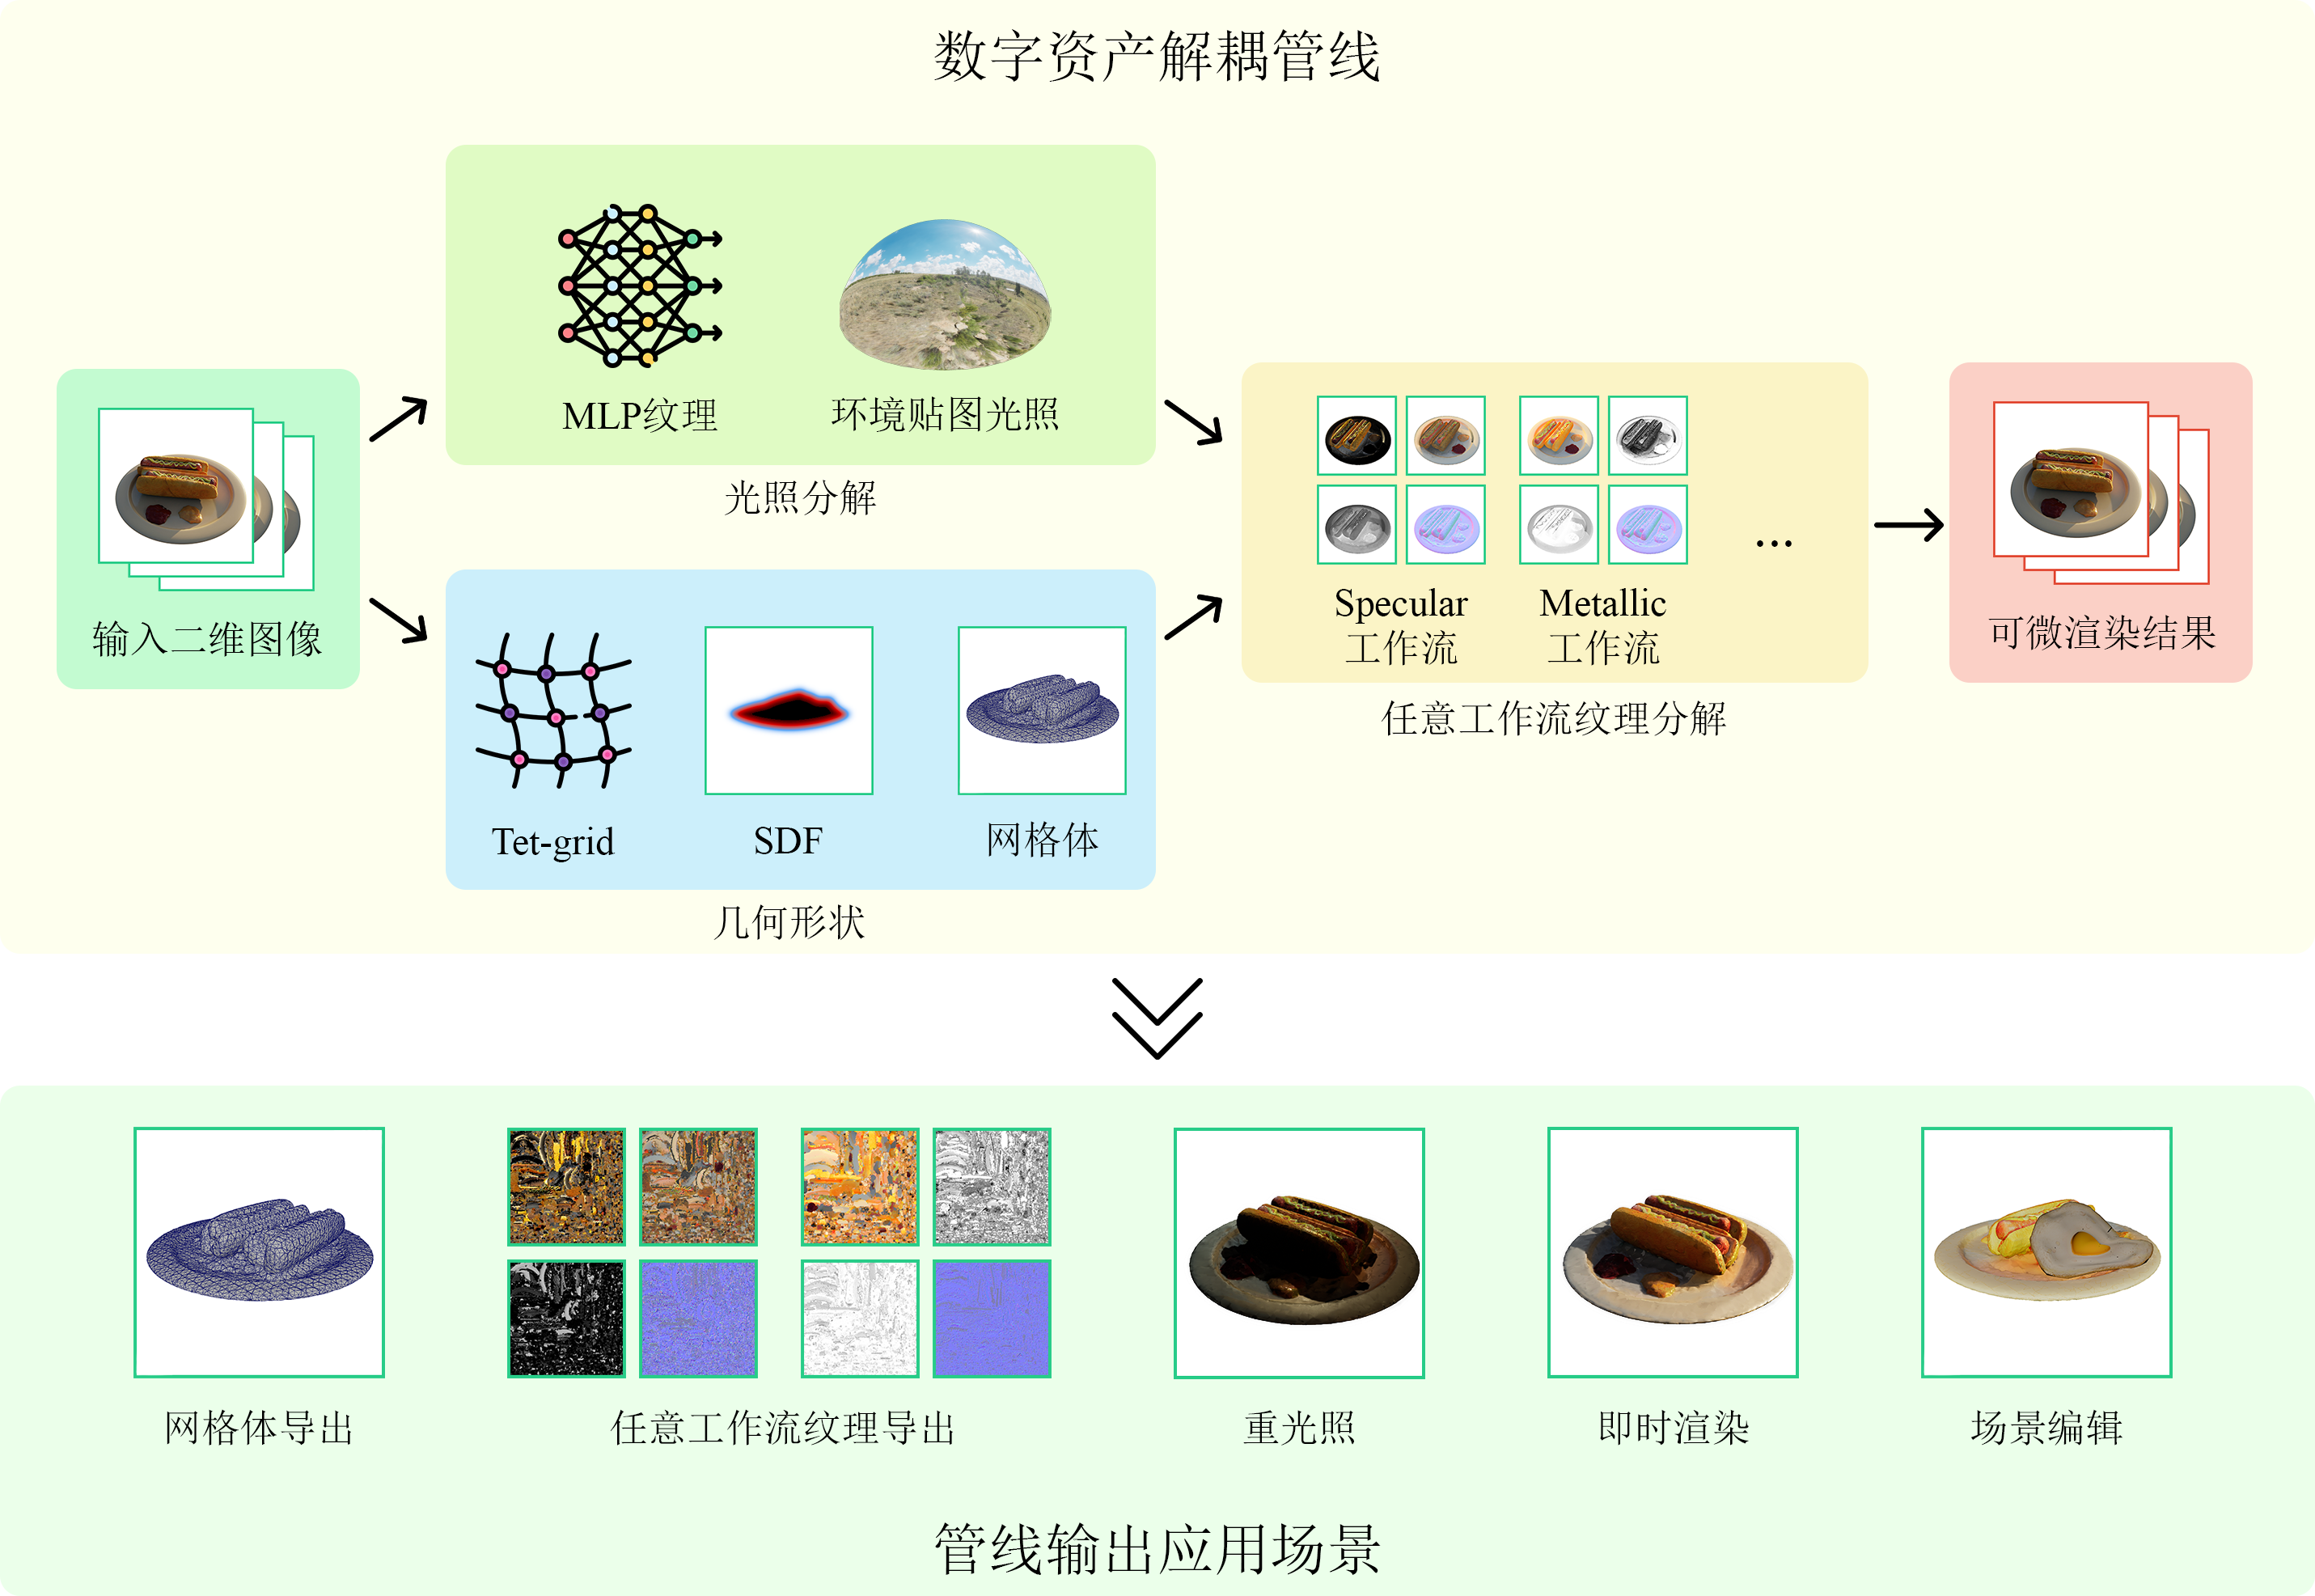
\includegraphics[width=1.0\linewidth]{Main_line_with_apply_with_big_zi.png}
  \caption{数字资产解耦管线与应用场景}
  \label{fig:main_pipe_line}
\end{figure}

\section{数字资产解耦问题分析}

工业界现有的资产大多归属于特定的工作流,而不同的着色模型也与工作流逐一对应,因此,
本文管线如果能够实现将任意工作流的数字资产转换到另一种任意工作流,即可将数字资产与任意的渲染技术相结合,
实现本文解耦的目标。

在技术路线上,本文选择了第二章中介绍的NeRF光照分解相关研究,在此基础上进行目标的实现。
NeRF光照分解管线所需的输入为场景的二维RGB图片,而待转换的数字资产可以通过渲染获得这些图片;
同时,该管线可以输出场景的几何形状和表面反射属性,与数字资产转换所需的输出类似。因此,
选择该技术开展研究和实现,对于本文的目标具备可行性。

但是,现有的工作为了提升几何重建效果,大多延续了NeRF中的隐式神经几何表示,
这导致管线的输出仅能用于重光照或新视角合成任务。而本文的目标是管线的输出能够无缝对接传统渲染器,
应用于即时渲染和下游编辑,因此本文需要对管线中的几何表示进行改造,使其输出显式网格体几何表示。
其次,现有管线受限于可微渲染的优化效率,多采用数据驱动的BRDF或固定规格的参数化BRDF作为反射属性表示,
无法满足本文使用任意工作流的需求,所以有必要针对反射属性部分重新设计,把指定工作流的纹理贴图作为输出。

基于以上分析,本文将目标进一步设置为,设计并实现一套管线,其输入为多张相机位姿已知、
光照环境及场景三维信息未知的二维RGB图片;输出为场景的几何形状和反射属性。其中,
输出的几何表示为网格体,反射属性为指定工作流对应的纹理贴图。

\section{管线设计}
本节将系统地介绍本文管线的设计与创新方法。首先,本文改进了几何表示方式,
通过一种显式隐式混合的方法,使得管线能够基于隐式表示进行优化的同时,
也能够直接输出显式网格表示的场景几何信息。随后,本文采用MLP纹理表示场景的表面反射属性,
这种设计带来了足够的灵活性,能够满足本文对任意工作流进行解耦的需求。
结合环境光照贴图作为光照技术进行可微渲染。在可微渲染中,本文允许使用任意的工作流表示
作为场景的反射属性的表示方法,使用渲染结果与原始输入计算损失,并将梯度传播到前述的几个阶段。
最后,本文管线输出网格体与纹理贴图,完成数字资产解耦的目标。接下来,本节将分别介绍以上部分。

\subsection{几何表示方式}

现有的隐式神经表示方法难以将生成结果直接用于下游编辑等任务,而传统的显式网格体则在重建效果上有所折损。
因此,本文采用了混合的几何表示方法DMTet\cite{shen2021deep},
其结合了SDF与网格体表示的优点,同时能够与传统渲染器无缝衔接。

根据本文在第二章的介绍,DMTet能够先通过SDF学习几何形状,随后以可微的方式转换为三角面网格体。
为了更高效地利用这种混合形状表示,本文进一步拓展了DMTet,引入了即时渲染中法线纹理这一技术,
在优化过程中依次使用SDF、网格体、法线纹理进行优化,接下来本文将详细介绍设计思路及实现方式。

在传统的渲染管线中,网格体在细节的精细程度取决于两个方面,首先是网格体的顶点数量,
对于细节较为丰富的区域,较高的顶点数量才能准确的还原精细结构;其次是网格体的拓扑结构,
其决定着顶点的连接和排布方式,理想的拓扑结构可以将顶点和边分配在形状发生突变的位置,
以实现相同的几何形状的同时使用尽可能少的顶点。所以,传统的数字资产在制作时通常会先完成一个较为精细的“高模”,
然后制作一个多边形数量较低的“低模”。在这一过程中,艺术家根据经验设置网格的拓扑结构,最后通过烘焙(Baking)
将“高模”中的细节以法线纹理的形式转移至“低模”中。同时,直接对网格体和法线纹理进行优化可能使得几何恢复任务变得更加困难,尤其是当凸起或凹陷既可能被网格表示,也可能被法线纹理表示时。因此,本文仅在优化的第三阶段中对法线纹理进行优化,而在前两个阶段不进行法线纹理优化。此策略能有效避免同时优化网格和法线纹理时可能出现的优化冲突问题。

基于以上这一流程,我们提出可以通过引入一个类似的逆向过程来提升几何估计的准确度,
从而改善3D重建的质量。本文设计的管线中将依次对SDF、网格体、法线纹理进行优化。首先,
SDF作为一种精细但计算效率较低的表示方式,视为“高模”,该阶段的优化目标是,发挥SDF在高频细节表示上的优势,
尽可能还原场景中的所有细节,以确保下一阶段中使用的网格具有足够的几何细节和拓扑结构。
随后,网格体的拓扑结构在经过初步的优化后将被固定,这一阶段的几何表示视为“低模”,
该优化阶段不断调整网格的顶点位置,使其精确包裹住场景的真实形状。最后,在网格体的形状确定后,
法线纹理的优化将用于表达细微的几何细节,以将场景的高频细节传递至最终网格模型中。

在具体实现中,由于SDF转换为网格体时不可避免地产生翻转或浮动的三角形面,因此本文采用了Liao等人\cite{Liao_2018}
提出的方法对DMTet的SDF值进行正则化。给定二元交叉熵损失函数$H$、Sigmoid函数$\sigma$和
符号函数$\mathrm{sign}(s_i)$,在满足$\mathrm{sign}(s_i)\neq\mathrm{sign}(s_j)$的条件下,
正则化项可以通过以下公式定义:
\begin{equation}\label{eq:Lreg}
L_{reg}=\sum_{i,j\in\mathbb{S}_e}\Bigl[H\bigl(\sigma(s_i),\mathrm{sign}(s_j)\bigr)+H\bigl(\sigma(s_j),\mathrm{sign}(s_i)\bigr)\Bigr]
\end{equation}
其中,$\mathbb{S}_e$表示四面体网格中边的集合,且条件为$\mathrm{sign}(s_i)\neq\mathrm{sign}(s_j)$。
该正则化项的直观解释是减少符号翻转的次数,从而简化表面,避免不必要的浮动几何体或内部几何结构。

随后,在对法线纹理优化的阶段中,本文没有强行固定网格体形状,但是为了避免上文所说的优化冲突问题,
本文选择使用损失函数限制法线纹理的变化,使网格体在初始化阶段保持法线纹理相对平滑,
尽可能地通过网格体形状表示场景细节。该损失函数可以由以下公式表示:

最后,本文观察到DMTet生成的网格体通常会将多个顶点挤压在一起,在局部细节上,
这有助于生成小块的平坦表面,但是在总体形状的表达上,这会导致大量的顶点和面被浪费,
无法有效表示形状。因此,本文使用如下损失函数,强制顶点之间分散开:

在后文的实验中,本文将通过定性的实验,验证该方法对于下游任务的适用性,
并通过定量的消融实验,解释并证明以上损失函数的工作原理及有效性。

表格示例:

\begin{table}
  \centering
  \caption{JSON VS XML 读取解析性能(Chrome V8)}
  \begin{tabular}{l|ccc}
    \toprule
    方法                       & 每秒操作次数 &  误差率     & 相对落后比例\\
    \midrule
    JSON.parse                & 28 ops/s   & \pm4.36\% &  0\% \\
    xml2js.parseString        & 12 ops/s   & \pm4.16\% &  65.52\% \\
    xml2js.parseStringPromise & 10 ops/s   & \pm6.23\% &  68.97\% \\
    \bottomrule
  \end{tabular}
  \label{tab:json-vs-xml}
\end{table}
